\chapter{Implementação de um Chatbot Baseado em Regras para Recuperação de Atas da UFRRJ}\label{chp:EXPERIMENTOS}

Este capítulo descreve a implementação da solução proposta, apresentando as ferramentas e bibliotecas escolhidas para cada componente, a forma como eles foram desenvolvidos e o ambiente necessário para sua execução.

\section{Escolha do Chatbot}

A implementação da camada conversacional partiu de uma decisão já justificada na Seção~\ref{sec:comparativo-chatbots}: a adoção de um chatbot baseado em regras, em vez de soluções fundamentadas em NLU, IA generativa ou modelos híbridos (Tabelas~\ref{tab:comparativo-chatbots} e \ref{tab:motivos-nao-adocao}). Essa escolha apoiou-se em três fatores combinados: o escopo fechado do problema, em que o usuário busca atas dentro de um conjunto pré-definido de critérios, favorece um fluxo de diálogo estruturado por regras condicionais; a ausência de orçamento para licenciamento de ferramentas torna preferível uma solução sem custo recorrente; e a necessidade de integração com uma API externa de busca exige suporte à execução de código dentro do próprio fluxo de conversa.

Dentro do universo de plataformas de chatbot baseado em regras, gratuitas e sem limite de uso quando hospedadas localmente, a Tabela~\ref{tab:comparativo-chatbots-regra} já comparou o Botpress v12 às alternativas Rasa, Rocket.Chat, Dialogflow e Flow XO. Diante desses critérios, optou-se pela plataforma \textbf{Botpress v12} \cite{botpress-about, botpress-docs}, ferramenta de código aberto, sem custo de licenciamento, que pode ser hospedada localmente. Além de fornecer uma interface visual para construção do fluxo de diálogo, o Botpress v12 permite a execução de ações em JavaScript diretamente no fluxo, recurso explorado neste trabalho para realizar chamadas HTTP à API REST do indexador de documentos, apresentado na Seção~\ref{sec:indexador-documentos}.

As seções seguintes detalham essa implementação: a Seção~\ref{sec:arquitetura-solucao} apresenta a arquitetura geral da solução; a Seção~\ref{sec:motor-busca} justifica a escolha do Elasticsearch como motor de busca; a Seção~\ref{sec:indexador-documentos} descreve o indexador de documentos desenvolvido em Node.js; a Seção~\ref{sec:mapeamento-criterios} detalha o mapeamento dos critérios de busca coletados pelo chatbot para a consulta ao Elasticsearch; e as Seções~\ref{sec:integracao-discord} e \ref{sec:ambiente-desenvolvimento} descrevem, respectivamente, a integração com o Discord e o ambiente de desenvolvimento necessário para a execução do sistema.

\section{Arquitetura da Solução}\label{sec:arquitetura-solucao}

A solução é composta por quatro componentes principais que se comunicam entre si: o \textbf{Botpress}, responsável pela interface conversacional e pelo fluxo de diálogo com o usuário; o \textbf{Elasticsearch}, responsável pelo armazenamento e pela busca por similaridade nas atas; o \textbf{indexador}, um servidor desenvolvido em Node.js responsável por extrair o conteúdo dos arquivos PDF e disponibilizá-lo ao Elasticsearch; e um \textbf{bot do Discord}, que oferece um canal alternativo de comunicação com o usuário, repassando as mensagens recebidas para o Botpress.

O fluxo de uma consulta ocorre da seguinte forma: o usuário envia uma pergunta pelo Botpress ou pelo Discord, que a encaminha ao indexador por meio de uma requisição HTTP; o indexador, por sua vez, monta uma consulta ao Elasticsearch e retorna os trechos das atas mais relevantes para a pergunta realizada.

\section{Escolha do Motor de Busca}\label{sec:motor-busca}

A escolha do motor de busca é uma das decisões mais relevantes neste trabalho, pois determina diretamente a forma como os documentos são indexados, consultados e ranqueados. Existem diversas soluções disponíveis para essa finalidade, cada uma com características, modelos de licenciamento e casos de uso distintos.

Abaixo falaremos brevemente dos motores de busca mais relevantes que encontramos:

\subsection{Apache Lucene}

O \textbf{Apache Lucene} \cite{lucene-docs} é uma biblioteca de busca de código aberto escrita em \textbf{Java}, amplamente utilizada como base para outros motores de busca. Diferentemente das demais soluções apresentadas nesta seção, o Lucene não opera como um serviço independente: ele é uma biblioteca que deve ser integrada diretamente ao código da aplicação, oferecendo maior controle sobre indexação, análise de texto e ranqueamento, porém exigindo maior esforço de desenvolvimento para sua utilização.

\subsection{Apache Solr}

O \textbf{Apache Solr} \cite{solr-docs} é um motor de busca de código aberto escrito em \textbf{Java}, construído sobre o Apache Lucene. Assim como o Elasticsearch, opera como um \textit{webservice}: mantém um servidor standalone que expõe uma API REST para indexação e consulta de documentos. Oferece recursos satisfatórios de busca textual, análise linguística e suporte a múltiplos formatos de documento, podendo ser amplamente adotado em sistemas corporativos e bibliotecas digitais.

\subsection{Vespa}

O \textbf{Vespa} \cite{vespa-docs} é uma plataforma de busca de código aberto desenvolvida originalmente pelo \textbf{Yahoo!} e posteriormente tornada pública \cite{vespa-site}, escrita predominantemente em Java e C++. Também opera como um \textit{webservice} distribuído, com diferencial no suporte nativo a busca vetorial (ANN) e ranqueamento com modelos de \textit{machine learning} (TensorFlow, PyTorch, ONNX), sendo utilizado por empresas como Spotify e Yahoo em aplicações de busca e recomendação em larga escala \cite{vespa-site}. Para o contexto deste trabalho, sua complexidade de configuração e infraestrutura seria desproporcional à coleção de atas institucionais da UFRRJ.

\subsection{Elasticsearch}

O \textbf{Elasticsearch} \cite{IBMElasticsearch} é um motor de busca e análise de código aberto, baseado na biblioteca Apache Lucene. Oferece recursos de busca escaláveis, podendo armazenar dados estruturados em formatos especializados para buscas otimizadas. Possui também um design de API RESTful, o que proporciona flexibilidade para a análise de dados e facilidade para a integração com aplicações. Trata-se de uma solução de busca textual rápida e amplamente disseminada, com escalabilidade horizontal e compatibilidade com diversas linguagens de programação, incluindo Java, Python, .NET, PHP, entre outras, e se destaca nesse cenário por combinar essas características com suporte a análise morfológica e o algoritmo BM25 para ranqueamento por relevância textual, permitindo a criação de analisadores personalizados a fim de aumentar a precisão da busca.

A escolha pelo Elasticsearch foi reforçada pela existência de trabalhos anteriores que buscam solucionar o mesmo problema no contexto institucional da UFRRJ. Em particular, o trabalho \textit{CapiBusca: um buscador de atas para o Departamento de Ciência da Computação} \cite{rigoni2023capibusca}, desenvolvido por Vinicius Nunes Rigoni em 2023, que já havia adotado o Elasticsearch como motor de busca para indexação e consulta das atas do DCC, validando a aplicabilidade também para o nosso cenário. Dessa forma, além de suas características técnicas, a existência de trabalhos anteriores no mesmo contexto permitiu concentrar os esforços deste trabalho na camada conversacional e na geração estruturada de consultas.

\section{Indexador de Documentos}\label{sec:indexador-documentos}

O indexador foi desenvolvido em \textbf{Node.js} \cite{nodejs-docs}, utilizando o framework \textbf{Express} \cite{expressjs-docs} para expor uma API REST com três rotas principais:

\begin{itemize}
  \item \texttt{/indexar}: percorre a pasta de documentos configurada, extrai o texto de cada arquivo PDF por meio da biblioteca \textbf{pdf-parse} \cite{pdfparse-npm} e envia o conteúdo extraído ao Elasticsearch;
  \item \texttt{/buscar}: recebe os critérios de busca informados pelo usuário (discente, docente, disciplina, processo, progressão, assunto, departamento e intervalo de datas) e monta dinamicamente uma consulta no formato \textit{Query DSL} do Elasticsearch, combinando cláusulas \texttt{match} e \texttt{match\_phrase} com pesos (\textit{boost}) distintos para cada campo, de modo a priorizar os critérios mais específicos;
  \item \texttt{/arquivos}: disponibiliza o acesso direto aos arquivos PDF originais por meio de uma rota estática.
\end{itemize}

A comunicação entre o indexador e o Elasticsearch é realizada por meio do cliente oficial \textbf{@elastic/elasticsearch} \cite{elasticsearch-js}, configurado com autenticação por usuário e senha e com validação do certificado TLS do servidor. As configurações sensíveis, como a URL do Elasticsearch, as credenciais de acesso, o caminho da pasta de documentos e o nome do índice utilizado, são definidas em variáveis de ambiente, carregadas por meio da biblioteca \textbf{dotenv} \cite{dotenv-npm} a partir de um arquivo \texttt{.env}, evitando que informações sensíveis fiquem expostas diretamente no código-fonte.

O processo de indexação foi projetado para ser resiliente a falhas pontuais: cada arquivo da pasta de documentos é processado individualmente, dentro de um bloco de tratamento de erros próprio, de modo que a falha na leitura ou na extração de texto de um arquivo específico (por exemplo, um PDF corrompido ou protegido) é registrada em log, mas não interrompe o processamento dos demais arquivos do lote. Arquivos dos quais não é possível extrair conteúdo textual são simplesmente ignorados, sem gerar um documento vazio no índice. Ao final do processamento de todos os arquivos, é solicitada uma operação de \textit{refresh} do índice no Elasticsearch, tornando os documentos recém-indexados imediatamente disponíveis para consulta, sem a necessidade de aguardar o intervalo padrão de atualização do índice.

O código-fonte completo do indexador, assim como dos demais componentes do sistema, está disponível no repositório do projeto no GitHub \cite{tcc-atas-ufrrj-repo}.

\section{Mapeamento dos Critérios de Busca para a Consulta}\label{sec:mapeamento-criterios}

Esta seção detalha a implementação do roteiro guiado de diálogo apresentado no Capítulo~\ref{chp:PROPOSTA}, descrevendo como cada critério de busca coletado pelo chatbot é convertido em parâmetros da requisição ao indexador e, em seguida, em cláusulas da consulta ao Elasticsearch.

\subsection{Critérios de Busca e Variáveis de Sessão}

O fluxo principal do chatbot, definido no arquivo \texttt{main.flow.json} do Botpress, conduz o usuário por sete critérios de busca, cada um armazenado em uma variável de sessão e, posteriormente, repassado como parâmetro do endpoint \texttt{/buscar} do indexador:

\begin{itemize}
  \item \textbf{Departamento} : nome ou sigla do departamento responsável pela ata, mapeado para os parâmetros \texttt{nomeDpto};
  \item \textbf{Disciplina} : nome da disciplina mencionada na ata, mapeado para o parâmetro \texttt{nomeDisciplinas};
  \item \textbf{Docentes} : nome de professores envolvidos no assunto da ata, mapeado para o parâmetro \texttt{nomeProfessores};
  \item \textbf{Período} : intervalo de datas da ata, convertido para os parâmetros \texttt{de} e \texttt{ate};
  \item \textbf{Discentes} : nome de alunos mencionados na ata, mapeado para o parâmetro \texttt{nomeDiscentes};
  \item \textbf{Processo/Edital} : número de processo ou edital, mapeado para o parâmetro \texttt{numeroProcessoEdital};
  \item \textbf{Progressão} : termo relacionado a progressões funcionais/acadêmicas, mapeado para o parâmetro \texttt{progressoes}.
\end{itemize}

Além desses sete critérios, o fluxo reserva um campo de \textbf{Outros Assuntos}, mapeado para o parâmetro \texttt{outrosAssuntos}, utilizado para descrições livres do tema da ata relacionados ao escopo acadêmico.

\subsection{Montagem da Consulta ao Elasticsearch}

O endpoint \texttt{/buscar} do indexador recebe os parâmetros correspondentes aos critérios informados pelo usuário durante a interação com o chatbot e monta dinamicamente uma consulta no formato \textit{Query DSL} do Elasticsearch. Os seis parâmetros definidos na constante \texttt{CAMPOS\_TEXTO} (\texttt{nomeDiscentes}, \texttt{nomeProfessores}, \texttt{nomeDisciplina}, \texttt{numeroProcessoEdital}, \texttt{progressoes} e \texttt{outrosAssuntos}) dão origem, cada um, a uma cláusula \texttt{multi\_match} pesquisada simultaneamente sobre quatro campos do documento indexado (\texttt{conteudo}, \texttt{texto\_da\_ata}, \texttt{texto} e \texttt{ementa}), com peso (\textit{boost}) próprio, definido de acordo com a especificidade do critério: \texttt{nomeDiscentes} e \texttt{nomeProfessores} recebem \textit{boost} 2; \texttt{nomeDisciplina} e \texttt{numeroProcessoEdital} recebem \textit{boost} 1,5; e \texttt{progressoes} e \texttt{outrosAssuntos} recebem \textit{boost} 1, com tolerância a erros de digitação (\texttt{fuzziness: AUTO}). O departamento (\texttt{nomeDepto}) é tratado em uma cláusula \texttt{multi\_match} própria, com \textit{boost} 1,5 e o operador \texttt{or} entre os termos da consulta, permitindo que o nome ou a sigla do departamento sejam reconhecidos de forma mais flexível. Todas essas cláusulas compõem o agrupamento \texttt{should} da consulta booleana, com \texttt{minimum\_should\_match} igual a 1, garantindo que ao menos um dos critérios informados seja correspondido.


A integração entre o indexador e o Elasticsearch é viabilizada pela própria API RESTful do motor de busca, que conta com clientes oficiais para diversas linguagens, como Java, Python, .NET, PHP e JavaScript/Node.js. Neste projeto, essa integração é feita por meio do cliente oficial \textbf{@elastic/elasticsearch} \cite{elasticsearch-js}, já apresentado na Seção~\ref{sec:indexador-documentos}, responsável por traduzir a estrutura de consulta montada pelo endpoint \texttt{/buscar} para requisições no formato \textit{Query DSL} aceito pelo servidor. A consulta resultante, no formato \textit{Query DSL} do Elasticsearch, é ilustrada a seguir.

\begin{figure}[H]
  \centering
  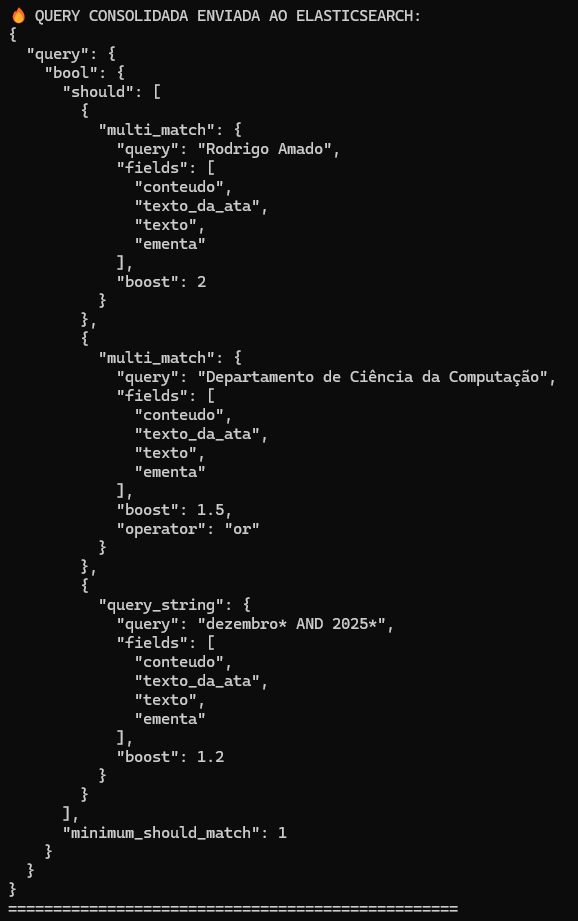
\includegraphics[width=0.6\textwidth]{imagens/queryExemplo.png}
  \caption{Query gerada com os seguintes parâmetros utilizados: Departamento, Discente e Período}
  \label{fig:queryExemplo}
\end{figure}

\subsection{Seleção e Exibição dos Resultados}\label{subsec:busca-proporcional}

A ação \texttt{buscarAtasProporcionais} é responsável por montar a requisição HTTP ao endpoint \texttt{/buscar} a partir das variáveis de sessão coletadas ao longo do roteiro de diálogo e por processar a resposta do indexador. Cada critério informado pelo usuário (departamento, disciplina, docentes, discentes, processo/edital, período, progressão e assunto geral) é incluído como parâmetro da \textit{query string} da requisição apenas quando preenchido; caso nenhum critério tenha sido informado, a busca não é realizada e a ação é encerrada antecipadamente, sinalizando que não houve resultado.

A requisição é feita por meio da biblioteca \textbf{axios} \cite{axios-npm}, com um tempo limite de cinco segundos. Os documentos retornados pelo indexador são ordenados de forma decrescente pelo \textit{score} de relevância atribuído pelo Elasticsearch, e os três primeiros colocados são selecionados para exibição. Para cada um desses documentos, a ação monta uma mensagem formatada contendo o título da ata, o \textit{score} (arredondado para duas casas decimais) e o \textit{link} de acesso ao arquivo PDF correspondente, servido pela rota \texttt{/arquivos} do indexador. Como o Botpress interpreta o caractere \textit{underscore} (\texttt{\_}) como marcação de itálico no formato Markdown, os títulos dos documentos --- que seguem o padrão de nomenclatura das atas, geralmente com \textit{underscores} no lugar de espaços --- têm esse caractere precedido por uma barra invertida antes da formatação da mensagem, evitando que o nome do arquivo seja exibido de forma incorreta ao usuário.

Caso a busca não retorne nenhum documento, é exibida uma mensagem informando que nenhuma ata foi encontrada para os critérios informados; caso ocorra um erro durante a requisição ao indexador (por exemplo, indisponibilidade do serviço), é exibida uma mensagem genérica de erro ao usuário.  O retorno das atas pelo buscador é exibido ao usuário conforme figura abaixo.

\begin{figure}[H]
  \centering
  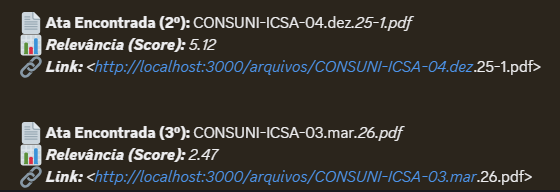
\includegraphics[width=0.8\textwidth]{imagens/retornoAtasExemplo.png}
  \caption{Retorno do bot com as atas encontradas para a busca realizada.}
  \label{fig:retornoAtasExemplo}
\end{figure}

\section{Integração com o Discord}\label{sec:integracao-discord}

Como canal alternativo de acesso ao chatbot, foi desenvolvido um bot para o \textbf{Discord} utilizando a biblioteca \textbf{discord.js} \cite{discordjs-docs}. Essa integração visa facilitar a utilização do bot pela comunidade acadêmica, visto que o DCC utiliza o discord como um dos canais oficiais de comunicação.

O bot escuta as mensagens enviadas em um canal específico e repassa o conteúdo para o Botpress por meio de uma requisição HTTP feita com a biblioteca \textbf{axios} \cite{axios-npm}, retornando ao usuário as respostas e os menus de opções gerados pelo fluxo de conversa.

\begin{lstlisting}[language=Java, breaklines=true, basicstyle=\footnotesize\ttfamily, frame=shadowbox, framexleftmargin=5mm, rulesepcolor=\color{gray}, caption={Escuta de mensagens no Discord e repasse ao Botpress via axios}, label={lst:discord-listener}]
client.on('messageCreate', async (message) => {
    if (message.author.bot) return;
    if (message.channelId !== CANAL_PERMITIDO_ID) return;

    let perguntaUsuario = message.content.trim();
    const usuarioId = message.author.id;

    try {
        const urlBotpress = `http://localhost:${BOTPRESS_PORT}/api/v1/bots/${BOT_ID}/converse/${usuarioId}`;
        const response = await axios.post(urlBotpress, { type: 'text', text: perguntaUsuario });

        // ... processamento da resposta do Botpress ...
    } catch (error) {
        console.error('Erro de comunicacao com o Botpress:', error.message);
        await message.reply('Ocorreu um erro ao consultar o assistente.');
    }
});
\end{lstlisting}

Quando a resposta do Botpress contém um menu de opções (campos \texttt{choices}, \texttt{options} ou \texttt{quick\_replies} da resposta da API), o bot extrai o título de cada opção e monta uma mensagem numerada no Discord. Essa lista de títulos é, então, armazenada em uma estrutura de memória temporária, associada ao identificador do usuário no Discord. Dessa forma, quando o usuário responde a um menu digitando apenas o número correspondente a uma das opções exibidas, o bot verifica se há uma lista de opções salva para aquele usuário e, em caso positivo, converte o número informado de volta para o texto original da opção escolhida, antes de repassar a mensagem ao Botpress. Esse mecanismo permite que o usuário interaja com os menus de opções do fluxo de diálogo digitando apenas números, sem que o Discord, diferentemente do Botpress, ofereça suporte nativo a botões ou outros elementos interativos de seleção. Essa ação visa facilitar a interação do usuário com o bot, sem que ele necessite escrever o nome da opção que deseja selecionar a cada interação. Abaixo temos um exemplo do menu exibido ao usuário.


\begin{figure}[H]
  \centering
  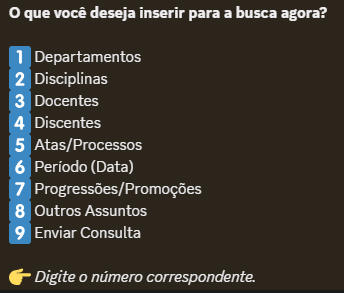
\includegraphics[width=0.5\textwidth]{imagens/exemploMenusNavegacao.png}
  \caption{Menu exibido ao usuário para facilitar a interação com o bot.}
  \label{fig:menusNavegacao}
\end{figure}


\section{Ambiente de Desenvolvimento}\label{sec:ambiente-desenvolvimento}

O indexador e o bot do Discord exigem o \textbf{Node.js} na versão 20 ou superior. Essa exigência decorre do uso do prefixo \texttt{node:} em módulos internos e de funcionalidades da \textit{Fetch API} (como a classe \texttt{File}), utilizadas internamente pelas dependências do projeto e disponíveis apenas a partir dessa versão; em versões anteriores do Node.js, a execução do indexador resulta em erros de módulo não encontrado. As dependências do projeto (\texttt{express}, \texttt{pdf-parse}, \texttt{@elastic/elasticsearch}, \texttt{dotenv}, \texttt{discord.js} e \texttt{axios}) são gerenciadas por meio do \textbf{npm} e descritas no arquivo \texttt{package.json}.

\section{Desempenho}\label{sec:desempenho}

O desempenho do sistema proposto se divide em duas etapas distintas, já descritas nas Seções~\ref{sec:motor-busca} e \ref{sec:indexador-documentos}: a indexação das atas e a busca propriamente dita. A indexação, realizada pela rota \texttt{/indexar} do indexador, extrai o texto de cada arquivo PDF por meio da biblioteca \textbf{pdf-parse} e envia esse conteúdo ao Elasticsearch, com um custo computacional proporcional ao volume de atas processadas em cada execução. Ainda assim, é uma etapa de pré-processamento, executada de forma antecipada e assíncrona em relação à interação do usuário com o chatbot. Uma vez concluída, os documentos ficam disponíveis para consulta, e o tempo gasto nesse processamento não chega a ser percebido pelo usuário durante a busca, já que esta ocorre sobre um índice pronto.

Quem realiza a busca em si é o Elasticsearch, motor descrito na Seção~\ref{sec:motor-busca} como uma solução de busca textual rápida, com escalabilidade horizontal e baseada em um índice invertido otimizado para a consulta \cite{IBMElasticsearch}. Por atuar sobre uma estrutura já indexada, sem precisar percorrer o conteúdo integral das atas a cada requisição, os resultados tendem a retornar de forma ágil ao usuário. A escalabilidade horizontal do Elasticsearch também sugere, em caráter qualitativo, que o sistema comportaria o crescimento do acervo de atas sem exigir uma reformulação estrutural do motor de busca.

Esse ponto, porém, precisa de uma ressalva: este trabalho não chegou a conduzir testes de desempenho formais sobre o sistema implementado. Não foram medidos tempos de resposta, taxas de indexação ou comportamento sob carga, e também não houve testes de \textit{benchmark} comparativos. As considerações anteriores sobre rapidez e escalabilidade partem, portanto, das características já conhecidas do Elasticsearch, e não de medições empíricas feitas neste trabalho ficando como ponto em aberto para avaliações futuras.

\section{Utilização do Chatbot}\label{sec:utilizacao-chatbot}

Conforme discutido nas Seções~\ref{sec:problema-gerar-consulta} e~\ref{sec:mapeamento-criterios}, o usuário possui um escopo fechado de critérios de busca, sendo possível pesquisar nas atas pelos seguintes temas: departamento, disciplina, docentes, discentes, período, número de ata, processo ou edital e progressões funcionais, além de ser possível informar outros assuntos relevantes no contexto acadêmico que não tenham sido mapeados nos critérios anteriores. Esta seção ilustra, por meio de capturas de tela reais da interação no Discord, como esse escopo se traduz na experiência do usuário.

\subsection{Abertura da Conversa}

Em sua primeira interação, o bot pergunta o nome do usuário a fim de tornar as interações seguintes um pouco mais pessoais (Figura~\ref{fig:interacaoInicial}).

\begin{figure}[H]
  \centering
  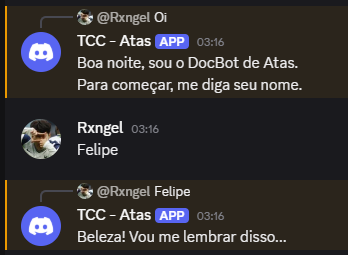
\includegraphics[width=0.5\textwidth]{imagens/interacaoInicialNome.png}
  \caption{Primeira interação com o bot, na qual é informado o nome do usuário.}
  \label{fig:interacaoInicial}
\end{figure}

Na interação seguinte, o bot exibe um menu com três opções, a partir do qual o usuário pode prosseguir diretamente para o início da busca, consultar instruções detalhadas de uso ou obter informações sobre o trabalho (Figura~\ref{fig:instrucoesUso}). Caso opte pelas instruções de uso, uma nova mensagem é enviada explicando como cada critério de busca deve ser informado, deixando claro que não é necessário preencher todos os campos, cabendo ao usuário informar apenas aquilo que for relevante para sua pesquisa; em seguida, o mesmo menu de três opções é novamente exibido, permitindo que o usuário prossiga para o início da busca.

\begin{figure}[H]
  \centering
  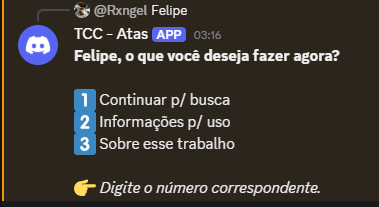
\includegraphics[width=0.5\textwidth]{imagens/instrucoesUso.png}
  \caption{Menu de opções inicial, a partir do qual é possível iniciar a busca ou receber instruções de uso.}
  \label{fig:instrucoesUso}
\end{figure}

\subsection{Navegação pelos Critérios de Busca}

Uma vez iniciada a busca, o bot apresenta um menu com os oito critérios de busca disponíveis, além da opção de enviar a consulta (Figura~\ref{fig:exemplo-menu-navegacao}). A cada critério informado pelo usuário, esse mesmo menu é exibido novamente, permitindo que outro critério seja preenchido ou que a consulta seja enviada; vale destacar que, como a consulta ao Elasticsearch é montada apenas ao final da interação, consolidando todas as informações fornecidas, o usuário deve informar todos os critérios desejados antes de optar por enviar a consulta, e não a cada critério individualmente.

\begin{figure}[H]
  \centering
  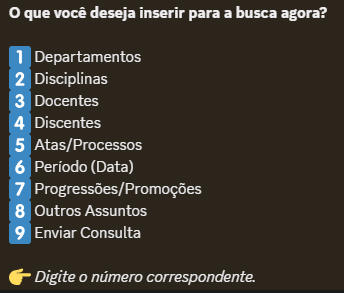
\includegraphics[width=0.5\textwidth]{imagens/exemploMenusNavegacao.png}
  \caption{Menu de opções para navegação entre os critérios de busca.}
  \label{fig:exemplo-menu-navegacao}
\end{figure}

\subsection{Consolidação das Informações e Envio da Consulta}

Ao selecionar a opção de enviar a consulta, o bot apresenta uma mensagem de consolidação com todas as respostas informadas até aquele momento, permitindo que o usuário confira exatamente o que será utilizado na busca antes de submetê-la (Figura~\ref{fig:respostas-consolidadas}). No exemplo ilustrado, foram informados os critérios de departamento, discente e período.

\begin{figure}[H]
  \centering
  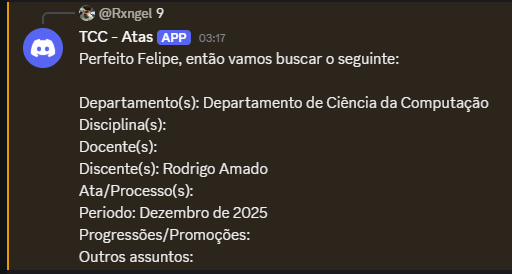
\includegraphics[width=0.7\textwidth]{imagens/respostasConsolidadas.png}
  \caption{Consolidação das respostas informadas pelo usuário antes do envio da consulta.}
  \label{fig:respostas-consolidadas}
\end{figure}

A partir dessas mesmas informações, o indexador monta a consulta no formato \textit{Query DSL} enviada ao Elasticsearch, conforme descrito na Seção~\ref{sec:mapeamento-criterios}. A Figura~\ref{fig:query-exemplo} ilustra a consulta efetivamente gerada para o exemplo da Figura~\ref{fig:respostas-consolidadas}: o nome do discente origina uma cláusula \texttt{multi\_match} com \textit{boost} 2, o nome do departamento origina uma cláusula \texttt{multi\_match} com \textit{boost} 1,5 e operador \texttt{or}, e o período origina uma cláusula \texttt{query\_string} com termos providos de curinga e \textit{boost} 1,2, todas agrupadas em uma cláusula \texttt{should} com \texttt{minimum\_should\_match} igual a 1.

\begin{figure}[H]
  \centering
  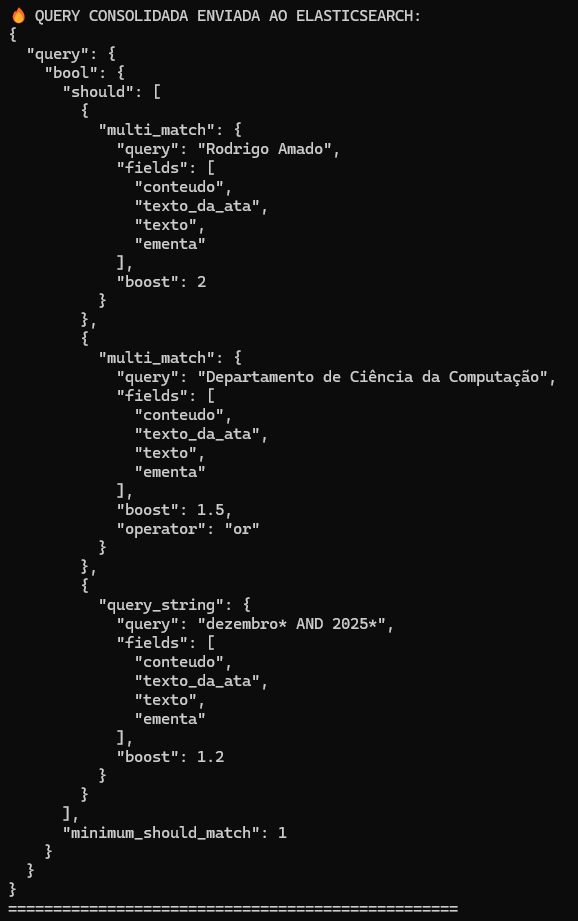
\includegraphics[width=0.5\textwidth]{imagens/queryExemplo.png}
  \caption{Query consolidada enviada ao Elasticsearch para o exemplo das Figuras~\ref{fig:respostas-consolidadas} e \ref{fig:retorno-atas}.}
  \label{fig:query-exemplo}
\end{figure}

\subsection{Exibição dos Resultados}

Após o envio da consulta, até três atas são exibidas ao usuário, ordenadas de forma decrescente de acordo com o \textit{score} atribuído pelo Elasticsearch, conforme descrito na Seção~\ref{subsec:busca-proporcional} (Figura~\ref{fig:retorno-atas}). Para cada ata, são exibidos o título do arquivo, o \textit{score} de relevância e o \textit{link} de acesso ao PDF correspondente, servido pela rota \texttt{/arquivos} do indexador.

\begin{figure}[H]
  \centering
  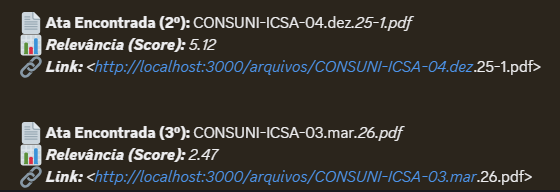
\includegraphics[width=0.7\textwidth]{imagens/retornoAtasExemplo.png}
  \caption{Retorno das atas encontradas, classificadas por \textit{score}.}
  \label{fig:retorno-atas}
\end{figure}